\begin{frame}
    \frametitle{Project Description}
    \begin{alertblock}{}
        We want to model the cellular communication as a system of different communication channels,
        where each node can communicate with others using LR pairs.
    \end{alertblock}

    \begin{alertblock}{}
        Each node is represented by a cell that has the following status $X_i = [R, x, y]$
        Where R is the rna expression counts and x and y are the euclidean spatial coordinates in
        respect ot a given reference point.
    \end{alertblock}
\end{frame}

\begin{frame}
    \frametitle{Schema}
    \normalsize  % global font reduction for the frame
    \begin{columns}
        \column{0.45\textwidth}
            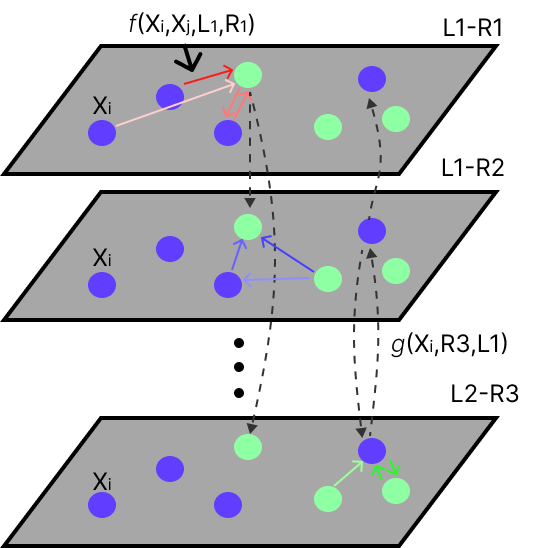
\includegraphics[width=\linewidth]{media/schema.png}

        \column{0.55\textwidth}
            \begin{block}{Intralayer links}
                The links can be thought as pairwise interactions between the cells and modeled by the function:
                $f(X_i,X_j,L_\alpha,R_\alpha)$
                Where $L_\alpha$ is the ligand in layer $\alpha$ and $R_\alpha$ is the receptor in layer $\alpha$.
            \end{block}
            \begin{block}{Interlayer links}
                The links can be thought as interactions between the Receptor in layer $\alpha$ and the Ligand in layer $\beta$ and modeled by the function:
                $g(X_i, R_\alpha, L_\beta$)
                Where the state of the cell $X_i$ is the same for both layers $\alpha$ and $\beta$.
            \end{block}
    \end{columns}
\end{frame}
\begin{frame}
    \frametitle{literature review}
    Still ongoing, but I did not find any paper that models the cellular communication using multilayer networks.
    Some ideas may be shared but I don't know.

    ....
\end{frame}
\begin{frame}
    \frametitle{Project milestones}
    \begin{enumerate}
        \item \textbf{Data collection}.
        \item \textbf{Prior knowledge} interpretation for both definition of comunications channels and relationship between comunication channels.
        \item ....
    \end{enumerate}
\end{frame}

\begin{frame}
    \frametitle{Data Collection}
    Al momento abbiamo a disposizione 2 dataset MERFISH/MERSCOPE
    \begin{itemize}
        \item \textbf{MERFISH - the one we have already seen}: 280'186 x 254 annotated, 2D, brain, from multiple not aligned slices of the MOp. 3 classes and 24 subclasses.
        \item \textbf{MERSCOPE}: 2'846'908 x 1'122 annotated, 3D, brain, from multiple samples. 34 classes and 338 subclasses.
        \item \textbf{Xenium}: .... we might need one. I have some references, but I don't have explored one yet.
        \item \textbf{Visium}: .... we might need one. I have many references, but I don't have explored one yet.
    \end{itemize}
\end{frame}

\begin{frame}
    \frametitle{Prior Knowledge}
    \begin{itemize}
        \item \textbf{NicheCompass}: curated Gene programs\break
            format: source str -> targets: List[str]
            \begin{itemize}
                \item GPLR - Ligand receptor pairs from Omnipath: [1042 entries]
                \item GPLRT - Ligand receptor target genes triplets from Nichenet: [1287 (325'898 single pair interactions) entries, with 1287 unique sources and 1157 unique set of targets and 12'694 unique targets (receptors and target genes)]
                \item GPES - Enzyme sensor pairs from Mebocost
                \item GPTFTG - Transcription factor target genen pairs from Collectri
            \end{itemize}
        \item \textbf{Liana - Mouse consensus}: Ligand-receptor pairs\break
            Nentries: 3989 format: source str -> target str (93.5+ KB)
        \item \textbf{Nichenet}: Union of ligand-receptor signalings and gene-regulatory pairs:\break
            Nentries: 8'229'548 format: sourcei (19724) str -> target(22503) str with weight float64 (251+ MB)
        \item \textbf{Omnipath}: Flow activity, general, ligand receptor, enzyme-sensor\break
            Nentries: 95'855 format: source str -> target str type\_source: str type\_target: str effect: int64
        \item \textbf{Collectri} Trascription factor target genes pairs:\break
            Nentries: 43'226 format: source str -> target str weight: float64 and others
    \end{itemize}
\end{frame}    
\begin{frame}
    \frametitle{Mathematical Framework}
    \begin{definition}{Tensor}
        A tensor is a multilinear function that maps objects defined in a vector space into other objects of the same type. Must be magnitude invariant under a change of basis.
        More generally, given a vector space $\mathcal{V}$ with algebraic dual space $\mathcal{V}^*$ over the real numbers $\mathbb{R}$.
        \begin{equation}
            M: \mathcal{V}^* \times \mathcal{V}^* \times \ldots \times \mathcal{V}^* \times \mathcal{V} \times \mathcal{V} \ldots \mathcal{V} \to \mathbb{R}
        \end{equation}
        Formally, we characterize a \textit{rank-mn} tensor $M_{j_1j_2...j_m}^{i_1i_2...i_n}$ that is \textit{m}-covariant and $\textit{n}$-contravariant.
    \end{definition}
\end{frame}

\begin{frame}
\frametitle{Mathematical Framework}
    \begin{definition}{Multilayer network}
        For a graph with \textit{N} nodes, the canonical covariant vectors $e_i(a)\in\mathbb{R}^{N}$ are $N$ rank 1 tensors with all entries to 0 except the $a-th$ entry, which is 1. 
        Similarly, for the canonical contravariant vectors.
        Let the adjacency tensor of a complex network be:
        \begin{equation}
            W_j^i=\sum_{a,b=1}^{N}w_{ab}e^i(a)e_j(b)=\sum_{a,b=1}^{w}w_{ab}E_j^i(ab)
        \end{equation}
        Where $w_{ab}$ is the weight of the edge between nodes $a$ and $b$.
        Similarly, let the adjacency tensor of a complex multilayer network be: 
        \begin{equation}
            M_{j\beta}^{i\alpha}=\sum_{a,b=1}^{N}\sum_{p,q=1}^{L}w_{ab}(pq)e^i(a)e_j(b)e^\alpha(p)e_\beta(q)
                                =\sum_{a,b=1}^{N}\sum_{p,q=1}^{L}w_{ab}(pq)E_{j\beta}^{i\alpha}(ab;pq)      
        \end{equation}
    \end{definition}
\end{frame}
\begin{frame}
    \frametitle{Mathematical Framework}
    \begin{definition}{SNXI decomposition}
        Different decompositions are possible, however, in multilayer adjacency tensors we can identify four tensors that encode distinct structural information:
        \begin{equation}
            m_{j\beta}^{i\alpha} = \mathbb{S}_{i\alpha}(M) + \mathbb{N}_{i\alpha}^j(M) + \mathbb{X}_{i\alpha}^{j\beta}(M)+\mathbb{I}_{i\alpha}^{\beta}(M)
        \end{equation}
        Where:
        \footnotesize
        \begin{itemize}
            \item $\mathbb{S}_{i\alpha}(M)$: \textit{self-interactions} tensor,interactions from a node to itself.
            \item $\mathbb{N}_{i\alpha}^j(M)$: \textit{endogenous interactions} tensor, interactions between distinct nodes belonging to the same layer.
            \item $\mathbb{X}_{i\alpha}^{j\beta}(M)$: \textit{exogenous interactions} tensor, interactions between distinct nodes belonging to distinct layers.
            \item $\mathbb{I}_{i\alpha}^{\beta}(M)$: \textit{intertwining} tensor, interactions from a node to its replicas in other layers.
        \end{itemize}
        \normalsize
        In our network, we are trying to model an \textit{Interconnected multiplex network}, which is of type \textit{SNI}.
    \end{definition}
\end{frame}
\begin{frame}
    \frametitle{Modeling Intralayer links}
    The intralayer links defines the strength of a communication channel between two agens (cells) (spatial locations)
    \begin{block}{}
        The intralayer links can be modeled by the function:
        \begin{equation}
            f(X_i,X_j,L_\alpha, R_\alpha) = \frac{X_{il} * X_{jr}}{\sqrt{(x_i - x_j)^2 + (y_i - y_j)^2}} 
        \end{equation}
        Where $X_{il}$ is the ligand expression of cell $i$ and $X_{jr}$ is the receptor expression of cell $j$. While,
        the denominator is the distance between the two cells in the layer.
        
        One, could also grid the space and evaluate the possible presence of the ligand $l$ in a specific position by using all cells
        as sources for the diffusion of such ligand.

        and other possible modelings that assume saturation of interaction.
    \end{block}
\end{frame}
\begin{frame}
    \frametitle{Modeling Interlayer links}
    Interlayer links defines the intracellular signaling pathways within a cell.
    \begin{block}{}
        The interlayer links needs to be modeled as the influence of a receptor as gene upstream of regulation of other ligands.

        We can surely start by looking at the correlation of a receptor that is upstream of regulatory pathways of another ligands
        as influence score.

        Then, we can move to somthing more complex that tries to filter indirect correlations.
    \end{block}
\end{frame}

